\documentclass[ignorenonframetext,plain]{beamer}
\setbeamertemplate{navigation symbols}{}

\newcommand{\vocab}{\mathcal{V}}
\newcommand{\corpus}{\mathcal{C}}
\newcommand{\pml}{p_{\textsc{ml}}}
\DeclareMathOperator*{\argmax}{argmax}
\newcommand{\score}{\mathit{score}}

\title{Learning to map strings to classes}
\subtitle{Comp 542 Natural Language Processing}
\author{Deniz Yuret}

\hypersetup{colorlinks,urlcolor=red}

\begin{document}

\begin{frame}
\maketitle
\end{frame}

\begin{frame}\frametitle{Applications}
\begin{itemize}
\item
  \href{http://en.wikipedia.org/wiki/Document_classification}{Document
    classification}: Text $\rightarrow$ \{ politics, religion, 
  sports, $\dots$ \}
\begin{itemize}
\item See \href{http://www-nlp.stanford.edu/IR-book}{Introduction to
  Information Retrieval} Chapter 13,
  \href{http://nlp.stanford.edu/fsnlp}{Foundations of Statistical NLP}
  Chapter 16 for an introduction.
\item Some datasets: \href{http://qwone.com/~jason/20Newsgroups}{20 Newsgroups},
  \href{http://www.daviddlewis.com/resources/testcollections/reuters21578}{Reuters
    21578}, 
  \href{http://www.ai.mit.edu/projects/jmlr/papers/volume5/lewis04a/lyrl2004_rcv1v2_README.htm}{Reuters
    RCV1}, and \href{http://www.cs.cmu.edu/~webkb/}{WebKB}.
\item More datasets available at \href{http://kdd.ics.uci.edu}{UCI
  KDD}, \href{http://archive.ics.uci.edu/ml/index.html}{ML},
  \href{http://csmining.org/index.php/data.html}{CSMining},
  \href{http://www.cs.cmu.edu/~TextLearning/datasets.html}{CMU}.
\end{itemize}
\item \href{http://en.wikipedia.org/wiki/Sentiment_analysis}{Sentiment
  analysis}: Text $\rightarrow$ \{ positive, negative \}
\begin{itemize}
\item
  \href{http://www.cs.cornell.edu/home/llee/opinion-mining-sentiment-analysis-survey.html}{Survey
    book} by Pang and Lee.
\item
  \href{http://www.cs.cornell.edu/people/pabo/movie-review-data}{Movie
    review data} by Pang and Lee.
\end{itemize}
\item \href{http://en.wikipedia.org/wiki/Anti-spam_techniques}{Spam
  detection}: Text $\rightarrow$ \{ spam, regular \}
\begin{itemize}
\item
  \href{http://www.aclweb.org/aclwiki/index.php?title=Spam_filtering_datasets}{Spam
  filtering datasets} from ACL Wiki.
\item \href{http://csmining.org/index.php/data.html}{Other datasets} from
  CSMining Group.
\item \href{http://archive.ics.uci.edu/ml/datasets/Spambase}{Spambase}
  from UCI machine learning repository.
\end{itemize}
\end{itemize}
\end{frame}

\begin{frame}\frametitle{String classification models}
We need to learn a function for classification from examples:\[
f: \mathcal{X}\rightarrow\mathcal{Y}
\] where $x\in\mathcal{X}$ is a string and
$\mathcal{Y}$ is a small list of classes.  This is typically done
by first learning a scoring function:\[
\score:\, \mathcal{X}\times\mathcal{Y}\rightarrow\mathbb{R}
\] and then finding $y\in\mathcal{Y}$ that maximizes the score:\[
f(x) = \argmax_{y\in\mathcal{Y}}\score(x, y)
\]
\end{frame}

\begin{frame}\frametitle{String classification models}
\[
f(x) = \argmax_{y\in\mathcal{Y}}\score(x, y)
\]
\begin{itemize}
\item Generative: $
\score(x, y) = \Pr(x, y)
$
\item Conditional: $
\score(x, y) = \Pr(y | x)
$
\item Max-Margin: $
\score(x, y) \mbox{ is not probabilistic.}
$
\item Unsupervised: $
\score(x, y) \mbox{ is learned without (x,y) examples.}
$
\end{itemize}
\end{frame}

\begin{frame}\frametitle{Naive Bayes: Generative Process}
To generate each (x, y) pair where $x = [x_1, x_2, \dots, x_n]$
consists of words $x_i$ from a vocabulary $\vocab$ and
$y\in\mathcal{Y}$ is a class:
\begin{itemize}
\item First pick $y\in\mathcal{Y}$ with probability $q_y$ (categorical
  distribution).
\item Then pick each word $x_i\in\vocab$ with probability\footnote{The
  length $n$ is assumed given, we could model it as well if
  desired.}\footnote{The probability of each word $x_i$ depends on the
  class $y$ but is conditionally independent of other words
  $x_{j\neq i}$.} $q_{x_i|y}$ (more categorical distributions).
\end{itemize}
\end{frame}

\begin{frame}\frametitle{Naive Bayes: Likelihood}
Given the Naive Bayes generative process, what is the probability of
generating a particular (x, y)?\[ \Pr(x, y) = q_y q_{x_1|y} q_{x_2|y}
\dots = q_y \prod q_{x_i|y}
\]
\end{frame}

\begin{frame}\frametitle{Naive Bayes: Estimation}
What are the maximum likelihood estimates for the Naive Bayes
parameters $Q$?\begin{eqnarray*}
q_y^* &=& \frac{\mbox{number of documents with class
    $y$}}{\mbox{number of documents}}\\
\\
q_{x_i|y}^* &=& \frac{\mbox{number of words $=x_i$ in class
    $y$}}{\mbox{number of words in class $y$}}
\end{eqnarray*}  
\end{frame}

\begin{frame}\frametitle{Naive Bayes: Issues}
\begin{itemize}
\item Maximum likelihood overfits: some words will have zero
  probability if never before observed with a class.
  \\ \textsl{Possible solution:} Use add-one (or other) smoothing.
  \\ \textsl{Accuracy on movie reviews:} 0.8125
\item Independence assumptions (bag-of-words view) too strong.
  \\ \textsl{Possible solution:} Use ngram models for each class.
  \\ \textsl{Accuracy on movie reviews:} 0.8450
\item Joint distribution $\Pr(x,y)$ may be difficult to learn and
  unnecessary if all we need is $\argmax\Pr(y|x)$.
  \\ \textsl{Possible solution:} Conditional model, learn
  $\Pr(y|x)$ directly.
  \\ \textsl{Accuracy on movie reviews:} 0.8565
\end{itemize}
\end{frame}

\begin{frame}\frametitle{Why conditional models?}
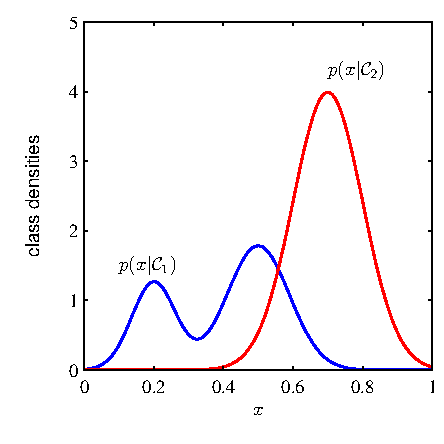
\includegraphics[width=.5\textwidth]{images/Figure1-27a.pdf}
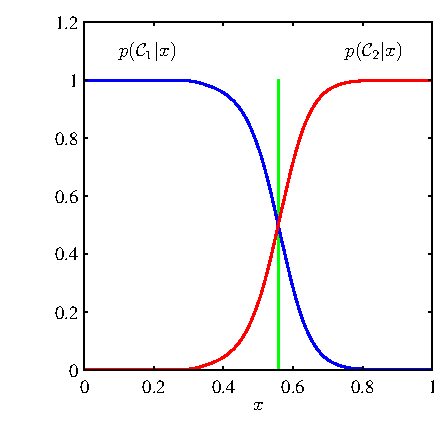
\includegraphics[width=.5\textwidth]{images/Figure1-27b.pdf}

\scriptsize Figure 1.27
(\href{http://research.microsoft.com/en-us/um/people/cmbishop/prml}
{Bishop, 2006}): Example of the class-conditional densities for two
classes having a single input variable $x$ (left plot) together with
the corresponding posterior probabilities (right plot). Note that the
left-hand mode of the class-conditional density $p(x|C_1)$, shown in
blue on the left plot, has no effect on the posterior
probabilities. The vertical green line in the right plot shows the
decision boundary in $x$ that gives the minimum misclassification rate.
\end{frame}

\begin{frame}\frametitle{Conditional log-linear models: Likelihood}
\begin{itemize}
\item Represent $(x, y)$ pairs using a feature vector function
  $\mathbf{g}: \mathcal{X} \times \mathcal{Y} \rightarrow
  \mathbb{R}^d:$ \[
\mathbf{g}(x, y) = [ g_1(x, y), g_2(x, y), \dots, g_d(x, y) ]^T
\]

\item Define score as linear combination of feature values: \[
  \score(x, y) = \mathbf{w}^T \mathbf{g}(x, y) = \sum w_i g_i(x, y)
\]

\item Maximizing score equivalent to maximizing conditional log-linear
  likelihood:
\begin{eqnarray*}
  p_w(y|x) &=& \frac{1}{z_w(x)}\exp \mathbf{w}^T \mathbf{g}(x, y) \\
  z_w(x) &=& \sum_{y'\in\mathcal{Y}} \exp \mathbf{w}^T \mathbf{g}(x, y') \\
  \argmax_{y\in\mathcal{Y}} p_w(y|x)
    &=& \argmax_{y\in\mathcal{Y}} \exp \mathbf{w}^T \mathbf{g}(x, y) \\
    &=& \argmax_{y\in\mathcal{Y}} \mathbf{w}^T \mathbf{g}(x, y)
\end{eqnarray*}
\end{itemize}
\end{frame}

\begin{frame}\frametitle{Conditional log-linear models: MLE}
Given training data $\{(x_1, y_1), (x_2, y_2), \dots \}$, the
maximum likelihood estimation for weights $\mathbf{w}$: \begin{eqnarray*}
\mathbf{w^*} &=& \argmax_\mathbf{w} \prod p_\mathbf{w}(y_i | x_i) \\
&=& \argmax_\mathbf{w} \sum \log p_\mathbf{w}(y_i | x_i) \\
&=& \argmax_\mathbf{w} \sum \mathbf{w}^T \mathbf{g}(x_i, y_i) - \log z_w(x_i)
\end{eqnarray*}
\begin{itemize}
\item There is no closed form solution.
\item The function is concave (unique maximum).
\item Algorithms like LBFGS can find the maximum quickly given the
  gradient.
\end{itemize}
\end{frame}

\begin{frame}\frametitle{Conditional log-linear models: Gradient}
\begin{eqnarray*}
  \ell(\mathbf{w}) &=& \frac{1}{N} \sum_{i=1}^N \left[ \mathbf{w}^T
    \mathbf{g}(x_i, y_i) - \log z_w(x_i) \right] \\ \frac{\partial
    \ell(\mathbf{w})}{\partial w_j} &=& \frac{1}{N} \sum_{i=1}^N
  \left[ g_j(x_i, y_i) - \frac{\sum_{y'\in\mathcal{Y}} g_j(x_i, y')
      \exp \mathbf{w}^T \mathbf{g}(x_i, y')}{z_w(x_i)} \right] 
  \\ &=& \frac{1}{N} \sum_{i=1}^N \left[ g_j(x_i, y_i) -
    \sum_{y'\in\mathcal{Y}} g_j(x_i, y') p_w(y'|x_i) \right]
  \\ &=& \frac{1}{N} \sum_{i=1}^N \left[ g_j(x_i, y_i) -
    \mathbb{E}_{p_\mathbf{w}(Y|X)} g_j(x_i ,Y) \right]
  \\ &=& \mathbb{E}_{\tilde{p}(X,Y)} g_j(X,Y) -
  \mathbb{E}_{\tilde{p}(X)p_\mathbf{w}(Y|X)} g_j(X,Y)
\end{eqnarray*}
\begin{itemize}
\item The first expectation is over the empirical distribution
  $\tilde{p}$.
\item The second expectation is over the model distribution $p_w$.
\item At the maximum the model expectation of each feature is equal to
  the empirical expectation.
\end{itemize}
\end{frame}

\begin{frame}\frametitle{Conditional log-linear models: Overfitting}
%% LSP pp.94
Example from (Smith, 2011): Consider a feature $g_6$ with value 1 on a
single training example $(x_9, y_9)$ and 0 for every other $(x, y)$
pair.
\end{frame}

\begin{frame}\frametitle{Conditional log-linear models: Regularization
    or MAP}

\end{frame}

\begin{frame}\frametitle{Conditional log-linear models under other
    names}
\begin{itemize}
\item Maximum entropy models: The parameters that maximize the
  likelihood of a log-linear model give us a distribution that also
  maximizes the entropy consistent with feature expectations.
\item Logistic regression: (actually a classification, not a
  regression technique) is a conditional log-linear model for binary
  outputs.
\item Naive Bayes: is a generative log-linear model (see
  \href{http://www.denizyuret.com/2010/11/naive-bayes-is-joint-maximum-entropy.html}{my
    blog post on this}).
%% linear svm vs logistic regression with l1/l2 prior, l1/l2 loss?
\end{itemize}
\end{frame}

\end{document}
